\section{Queue Module}
\label{sec:queue}
Queue is a utility module which is used by other modules to send messages from one to another. As shown in Figure \ref{fig:architecture}, there are 3 queues in BGPMon.
\begin{itemize}
	\item{\emph{ Peer Queue:} It is used by peering module to send internal messages with type 1,2,4 and 6 to the rib and labeling module.}
	\item{\emph{ Label Queue:} It is used by rib and labeling module, periodic module and main module to send all eight types of internal messages to XML generation module. }
	\item{\emph{ XML Queue:} It is used by XML generation module to send XML messages to client management module which in turn sends them to client applications.}
\end{itemize} 
Each of them is a running instance of queue module. They are created by main module during the initial phase of BGPmon and then used by other modules.

The queue module is build on a circular array and each item in this array contains a generic pointer which points to the real message. In this way we can make queue module generic enough to hold all kinds of messages. It also keeps track all the readers and writers. The main data structure of queue module will be introduced in subsection \ref{sub:queue:struct}.

The queue module implements a Readers/Writers pattern where multiple threads may access the same queue simultaneously, some reading and some writing. We call the reading thread reader and the writing thread writer. Each message written by a writer is available to all the readers and a message can be deleted from the queue only after all the readers read it. A key design issue is the locking mechanism to synchronize access to the share data structure in the queue among all threads.  The details of thread synchronization will be discussed in subsection 
\ref{sub:queue:sync}.
 
The biggest challenge in the design of queue module is to avoid being overwhelmed with limited queue length.  There are two situations we need to address: 1) writers write too fast, and 2) Readers read too slow. We will discuss how to address these two situations in subsection \ref{sub:queue:control}.
 
 
\subsection{\label{sub:queue:struct}{Main Data Structure}}
The main data structure of queue module is called 'Queue'. It consists of four parts:
\begin{itemize}
	 \item{\emph{ General Substructure:} It holds the general information for this queue such as the queue's name, its mutex lock and some logging information. See the details in \ref{sub:queue:struct:general}.}
	\item{\emph{ Items Substructure:} It contains all the data of the queue. It implements a circular array. See the details in \ref{sub:queue:struct:items}.}
	\item{\emph{ Readers Substructure:} It contains the information of all readers of the queue. For example, the sequence number of the next unread item for each reader needs to be maintained here. See the details in \ref{sub:queue:struct:readers}.}
	 \item{\emph{ Writer and Pacing Substructure:} It is used to track all the writers in order to pace them when needed. And some other information needed for pacing are also included here such as pacing on/off threshold.  See the details in \ref{sub:queue:struct:writers}.}
\end{itemize}  

\subsubsection{\label{sub:queue:struct:general}{General Substructure}}
The general substructure has the following fields:
\begin{itemize}
	\item{\emph{name:} It is the name of the queue. In BGPmon, the name of peer queue is 'PeerQueue', the name of lable queue is 'LabelQueue' and the name of XML queue is 'XMLQueue'. }
	\item{\emph{ queueLock:} It is a pthread mutex lock which is used for thread synchronization.}
	\item{\emph{ queuecond:} It is a pthread condition variable which is used to notify a reader when the new item gets wrote.}
	\item{\emph{ logging related fields:} A group of logging related fields such as the historical max number of messages, the historical max number of readers and the historical max number of writers.}
	\end{itemize}
Figure \ref{fig:queue:struct:general} shows the details.
\begin{figure*}
\centering
\scalebox{1}{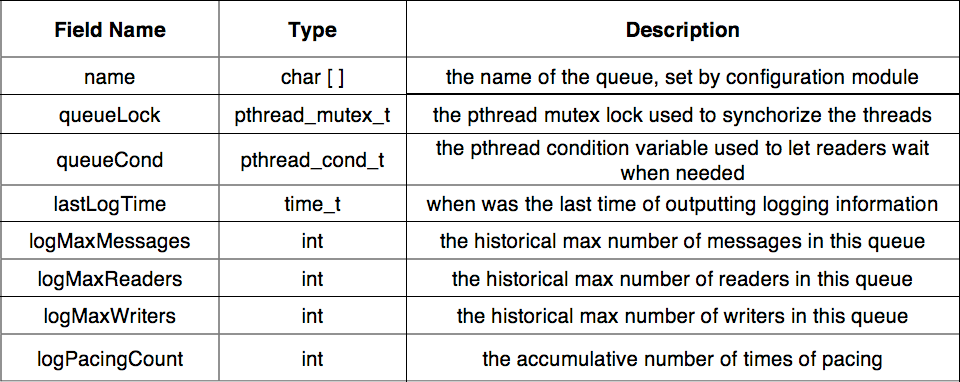
\includegraphics{figs/QueueStructGeneral.pdf}}
\caption{ General Substructure of Queue}
\label{fig:queue:struct:general}
\end{figure*}
	 

\subsubsection{\label{sub:queue:struct:items}{Items Substructure}}
Items substructure maintains a circular array of items which is the heart of queue module. 
Each item is defined as a 'QueueEntry' structure which has the following two fields:
\begin{itemize}
	\item{\emph{count:} It indicates how many readers haven't read it.   This reference count decrements by one after one reader reads this item. If the reference count of a item is zero, this item can be reclaimed by the queue module. Otherwise this item cannot be reclaimed.}
	\item{\emph{messageBuf(void *):} It points to the real data buffer of this item. The data buffer must be created by writers and be passed into queue module.}
\end{itemize}
Items substructure has the following five fields:
\begin{itemize}
	  \item{\emph{head:} It is the sequence number of the oldest item in the queue. It means at least one reader hasn't read this item. The 'head' is incremented after the oldest data item is read by the last reader. }
	  \item{\emph{tail:} It is the sequence number of the next available item in the queue. It is incremented by writing a new message into the queue. }
	  \item{\emph{items:} It is an array of items. Each item is a 'QueueEntry' structure.}
	  \item{\emph{ copy:} It is a callback function. If a reader reads a item and it is not the last reader for this item, the callback function will be called to return a copy of this item to the reader. If a reader is the last one of a item, this item will be returned directly. This allows the reader to always free the returned item after processing it without knowing the details of queue. }
	  \item{\emph{ sizeof:} It is a callback function. Based on 'QueueEntry' structure, we know the size of a item depends the size of its data buffer. This function is used to get the size of a data buffer in bytes. As the data format is queue specific, the sizeof function is provided by the queue creator.}
\end{itemize}
In order to avoid drop any messages in the queue, the different between 'head' and 'tail' must be smaller than 'max' field. Note 'head' and 'tail' are all sequence numbers, not subscripts of array. A sequence number(seq) is long integer and is a logical subscript of the queue. The subscript to access the physical array can be calculated by seq \% max.
Figure \ref{fig:queue:struct:items} shows the details of this substructure.
\begin{figure*}
\centering
\scalebox{1}{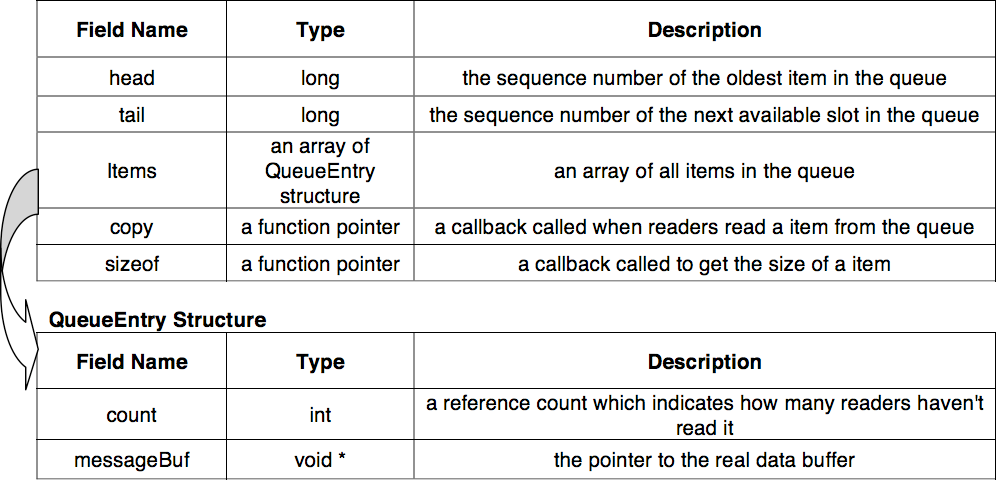
\includegraphics{figs/QueueStructItems.pdf}}
\caption{ Items Substructure of Queue}
\label{fig:queue:struct:items}
\end{figure*}
	 

\subsubsection{\label{sub:queue:struct:readers}{Readers Substructure}}
This substructure is used to track all the readers. It has the following three fields:
\begin{itemize}
	\item{\emph{readerCount:} It is the current number of readers. }
	\item{\emph{nextItem:} It is an array of sequence numbers for all the readers. This array is indexed by reader ID and each sequence number indicates the next unread item in the queue for the corresponding reader. For example, nextItem[6] is the sequence number of the next unread item for the reader with ID 6. The length of this array equals the max number of readers. }
		\item{\emph{itemsRead:}  This array is indexed by reader ID and each element indicates total items read by the corresponding reader. For example, itemsRead[6] is the number of total read items by the reader with ID 6. The length of this array also equals the max number of readers. }
\end{itemize}	
Note the readers of the same queue might have different next item. 


Figure \ref{fig:queue:example} shows an example of the queue which can help us understand the items substructure and readers substructrure.
\begin{figure}[!htb]
\centering
\scalebox{0.44}{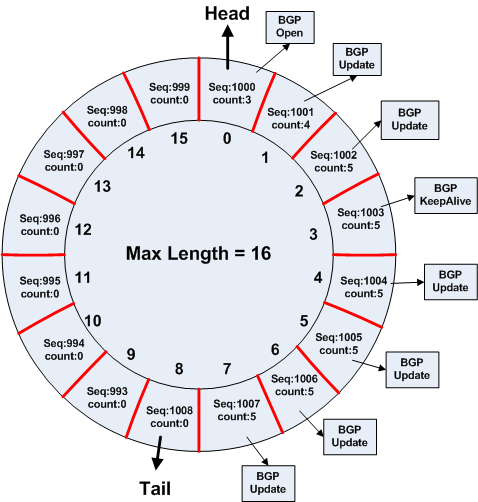
\includegraphics{figs/QueueExample.png}}
\caption{ An Example of Queue}
\label{fig:queue:example}
\end{figure}
In this example, there are a queue with max length 16 and 5 readers. The items substructure looks like this:
\begin{itemize}
	\item{\emph{head:} is 1000 which is sequence number of the oldest item. The count of that item is 3 which means there are three readers haven't read it. }
	  \item{\emph{tail:} is 1008 which is sequence number of the next available item for the new message. }
	  \item{\emph{items:} It is an array of 16 items. 8 of them are in use. }
	  \begin{itemize}
	  	\item{The item with sequence number 1000 has a reference count as 3 which means 3 readers haven't read it.}
		 \item{The item with sequence number 1001 has a reference count as 4 which means 4 readers haven't read it.}
		 \item{All the others item with sequence number from 1002 to 1007 has a reference count as 5 which means all 5 readers haven't read it.}
	\end{itemize}
\end{itemize} 

The corresponding readers substructure is as follows:
\begin{itemize}
	\item{\emph{readerCount:} is 5 which means there are 5 readers.}
	  \item{\emph{nexItem[0]:} is 1000 which means the next item for the reader 0 is 1000 .}
	   \item{\emph{nexItem[1]:} is 1000 which means the next item for the reader 1 is 1000 .}
	    \item{\emph{nexItem[2]:} is 1000 which means the next item for the reader 2 is 1000 .}
	     \item{\emph{nexItem[3]:} is 1001 which means the next item for the reader 3 is 1001 .}
	      \item{\emph{nexItem[4]:} is 1002 which means the next item for the reader 4 is 1002 .}
	      
	     	  \item{\emph{itemsRead[0]:} is 0 which means reader 0 hasn't read anything .}
	   \item{\emph{itemsRead[1]:} is 0 which means reader 1 hasn't read anything.}
	    \item{\emph{itemsRead[2]:} is 0 which means reader 2 hasn't read anything.}
	     \item{\emph{itemsRead[3]:} is 1 which means reader 3 has read 1 items.}
	      \item{\emph{itemsRead[4]:} is 2 which means reader 4 has read 2 items.} 
\end{itemize} 


\subsubsection{\label{sub:queue:struct:writers}{Writers and Pacing Substructure}}
This structure is used to track the writing rate of all the writers and pace them when needed. It has the following fields:
 \begin{itemize}	
 	\item{\emph{writerCount:} It is the number of current writers.}
	  \item{\emph{tick:} It is the start time of the current pacing interval.}
	  	\item{\emph{readCount:} It is used together with 'tick' to count how many messages are read in one interval by all the readers. }
	\item{\emph{writeCounts:} It is an array of counts for all the writers. One count is for each writer which is used together with 'tick' to count how many messages are written in one interval. The length of this array equals the max number of writers.}
	\item{\emph{writesLimit:} It is how many messages are allowed to be written in the queue by each writer in one interval when pacing is turned on. }
	\item{\emph{pacingFlag:} It is set to TRUE if pacing is turned on. It is set to FALSE if pacing is turned off.} 
\end{itemize} 
Figure \ref{fig:queue:struct:writers} shows the details of this substructure.
\begin{figure*}
\centering
\scalebox{1}{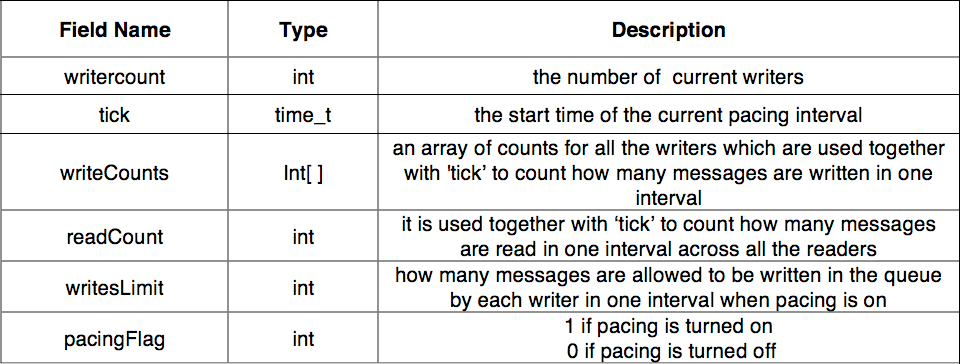
\includegraphics{figs/QueueStructWriters.pdf}}
\caption{ Writers and Pacing Substructure of Queue}
\label{fig:queue:struct:writers}
\end{figure*}
In the subsection \ref{sub:queue:control}, we will discuss how pacing works by using this substructure in detail.
 
\subsection{\label{sub:queue:sync}{Thread Synchronization}}
In BGPmon, there are multiple writers that write messages into one queue and multiple readers that read messages from the same queue. As each read/writer is a separate thread, the thread synchronization is very important for the queue. In our design we use mutex lock and condition variable to manage the thread synchronization. Basically the writer needs to lock the queue by obtaining 'queuelock' in general substructure before it writes a message and unlock the queue by release  'queuelock'  after it writes a message. Similarly the reader needs to lock the queue before it reads a message and unlock the queue after it reads a message.

When a reader exhausts the messages in the queue, it must wait for new messages while other readers or writers still need to continue their reading or writing. In our design, if a reader wants to read a message from the queue and successfully locks the queue by obtaining 'queuelock', it will do the following checks:
 \begin{itemize}	
 	\item{If there are some new messages available for it to read, it will read the oldest one and unlock the queue.}
	\item{Otherwise, it unlocks the queue and waits on the condition variable 'queueCond' to lock the queue again. If any writer writes any new messages into the queue, the queue will broadcast this condition to all the waiting readers.}
\end{itemize} 

\subsection{Interface Functions}
In the queue module, there are only two interface functions which can be used by other modules.
 \begin{itemize}	
 	\item{\emph{readQueue:} It is used to read a message from queue by giving a queue ID, reader ID and a pointer which points to the result data buffer. The return value of 'readQueue' is the number of remaining messages of this reader. It may return READER\_SLOT\_AVAILABLE if this reader has ceased. See details in \ref{sub:queue:control:adjust}}.
	\item{\emph{writeQueue:}  It is used to write a message into queue by giving a queue ID, writer ID and a pointer which points to the written message. It returns 0 if successes.}
\end{itemize}  

\subsection{\label{sub:queue:control}{Stream Control}}
In our design, the queue removes a message until all the readers read it. As a result there are two things we can do in order to prevent a queue being overwhelmed.
\begin{itemize}
	\item{\emph{Pacing writers:} The queue paces the writers according to the average reading rate across all the readers. For example the queue is almost full and there are 4 readers and 2 writers. If each of reader can read 8 messages per second averagely, we should limit the writing rate of each writer to 8/2 = 4 in order to avoid overwhelm the queue.  See details in \ref{sub:queue:control:pacing}.}
	\item{\emph{Adjust slow readers:} In some cases pacing writers doesn't work, the queue needs to adjust the slow readers. For example, the queue is almost full and there are 4 readers and 2 writers. If 3 of the 4 readers can read 8 messages per second but one of them can only read 2 message per second. As a result, the average reading rate across the 4 readers is 6.5 messages per second. In this case, even pacing is turned on and each writer is limited to write 6.5/2 = 3.25 messages per second the queue will still be overwhelmed because the slowest reader cannot read 3.25 messages per second. That's why in this case the queue has to adjust the slowest reader by skipping its unread items. See details in \ref{sub:queue:control:adjust}.}
\end{itemize} 

\subsubsection{\label{sub:queue:control:pacing}{Pacing Writers}}
In our design, the queue utilization(from 0\% to 100\%) is used to determine when to turn on pacing.  When the queue utilization exceeds a configurable threshold(PacingOnThreshold), pacing is turned on until the queue utilization drops below a configurable threshold(PacingOffThreshold).  The reason why we have two thresholds here is this allows the queue to reach a steady state rather than oscillate in and out of pacing.
During the pacing period, the objective is to make the writers write at a pace that matches the average reader. More specifically, in each configurable interval(PacingInterval) the queue limits the number of writes from each writer according to the average number of reads by all readers. 
In order to do this,  when a new interval starts we need to predict the number of reads by all readers in this new interval and then use this value to pace the writers in this new interval.   
The pacing related logic related to the 'readQueue' function is as follows:
\begin{enumerate}
	\item{Check if a new interval starts}
		\begin{enumerate}
		\item{If yes,  update the 'writesLimit' using exponential weighted moving average(EWMA):}
				\begin{enumerate}
					\item{Calculate the new 'writesLimit' by this formula. Note 'alpha' is configurable, 'writesLimit' is the number if writes allowed per writer in the new interval, 'averageReads' is the average number of reads by all readers in the past interval and 'writerCount' is the number of writers.}						
								\begin{eqnarray*}
writesLimit&=& (1-alpha) * writesLimit + \\ 
alpha *  \frac{averageReads}{writerCount}
						\end{eqnarray*}
						\item{If new 'writesLimit' is larger than half of the remaining queue, use half of the remaining queue as the new 'writesLimit'. }
					\item{If new 'writesLimit' is smaller than a configurable 'minWritesLimit', use 'minWritesLimit' as the new 'writesLimit'. }
				\end{enumerate}
		\item{Otherwise, do nothing.}
		\end{enumerate}
		\item{Check if needs to turn off pacing by compare the queue utilization with the configurable threshold(PacingOffThreshold).}
		\begin{enumerate}
			\item{If the queue utilization is smaller, set the 'pacingFlag' field as FALSE. }
			\item{Otherwise, do nothing.}
		\end{enumerate}
\end{enumerate}
Note this logic will be executed every time a reader calls 'readQueue'.

The 'writeQueue' function starts with the same pacing related logic as 'readQueue'. But after that, it needs to limit the number of writes per interval according to the 'writersLimit' field when pacing is enabled. This additional step inside the 'writeQueue' function is as follows:
\begin{enumerate}	
	\item{Check if needs to turn on pacing by compare the queue utilization with the configurable threshold(PacingOnThreshold).}
			\begin{enumerate}
			\item{If the queue utilization is larger, set the 'pacingFlag' field as TRUE. }
			\item{Otherwise, do nothing.}
			\end{enumerate}
			
	\item{Check if 'pacingFlag' is set to TRUE. }
		\begin{enumerate}
		\item{If yes,  do the following checks:}
				\begin{enumerate}
					\item{If 'writeCount[writerID]' is larger than 'writesLimit', sleep until a new interval starts.}
					\item{Otherwise, do nothing.}
				\end{enumerate}									
		\item{Otherwise, do nothing.}
		\end{enumerate}
\end{enumerate}
This logic will be executed every time a writer calls 'writeQueue'.
  
\subsubsection{\label{sub:queue:control:adjust}{Adjust Slow Readers}}
Pacing prevents the queue from being overwhelmed if the readers are uniformly able to read the messages at the same rate.  In the case of a slow reader, the queue utilization will still continue to grow.  When the queue utilization reaches the maximum, the responsible reader is adjusted by skipping all its unread items.
This logic is mainly implemented in the 'writeQueue' function.
\begin{enumerate}
	  \item{Check if the queue is full.}
	     \begin{enumerate}
	     \item{If it is full, find the slowest reader and adjust it by skipping all its unread items. For each reader, check the nextItem[readerID] as follows:}
	     		\begin{enumerate}
	     			\item{ If nextItem[readerID] equals to 'head', adjust this reader as mentioned.}
			\end{enumerate}	
	     \end{enumerate}
\end{enumerate}

In the 'readQueue' function, suppose the queueID, readerID and a pointer is passed in from a caller.
\begin{enumerate}
	\item{If head <= nextItem[readerID] < tail , pass the oldest message to the caller via the pointer and return the number of remaining messages.}
	\item{If nextItem[readerID] >= tail,block the caller until a new message is written into the queue. }
	\item{If nextItem[readerID] = READER\_SLOT\_AVAILABLE , it means the reader has ceased and return READER\_SLOT\_AVAILABLE to the caller.}
\end{enumerate}
If a caller receives READER\_SLOT\_AVAILABLE from 'readQueue', that means the corresponding reader has ceased. Then the caller may need to close thread and release resources in this case.

\subsection{Design Philosophy}
The most important design issue here is how to handle slow readers.  As we discussed, it is essential that some action be taken to address the problem of slow readers. If no action is taken,  a slow reader can cause the queue to overflow and eventually data would be dropped.   This is particularly problematic if most readers could read at a high rate and receive all the data, but a few slow readers fill the queues and cause data loss.   

In the previous design, our solution is to identify and then terminate the slow readers.  However, by doing that a potential problem is that the slow reader may simply re-connect and thus drive the overall system into a state of persistent oscillation.    The system runs well until the slow reader joins.   The slow reader then causes queues to build up and the reader is eventually killed.   The queue then quickly drains when the slow reader is killed.   Note that the queue contains at least one update that has been read by everyone except the slow reader.    When the slow reader is killed, that update can be discarded.    In our experiments thus far, a typical slow reader has hundreds of updates that are waiting only for the slow reader;  killing the slow reader immediately removes these updates and frees hundreds of slots in the queue.   But oscillation occurs if the slow reader immediately connects.    The queue of unread updates begins to build again as soon as the slow reader joins and the cycle repeats.   One can easily imagine a poorly written slow reader that automatically reconnects anytime it is disconnected.

An alternate approach is to better manage, but not kill the slow readers.   In current design, the slow reader is not deleted from the system.   Instead, slow readers are forced to skip messages.     From a queuing standpoint, the effect is similar to killing the slow reader and works as follows.   When BGPmon determines a reader is reading messages too slowly,  all messages that have yet to be read by that slow reader are immediately marked as read.    In this case the slow reader misses several messages, but it is allowed to continue. 



